\documentclass[border=10pt]{standalone}
\usepackage{tikz}
\usetikzlibrary{arrows.meta, calc}

\begin{document}
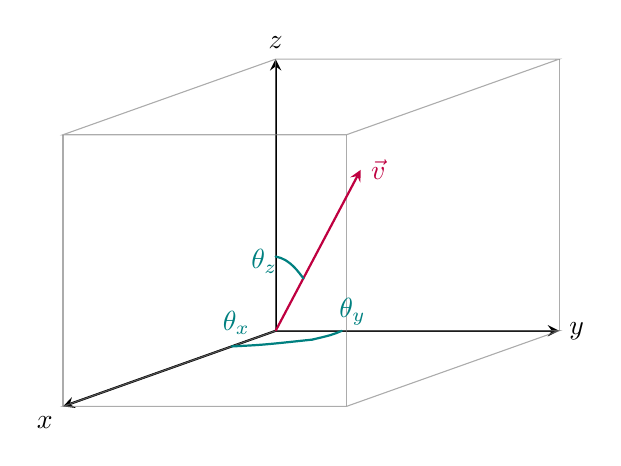
\begin{tikzpicture}[
    x={(-0.9cm,-0.32cm)},
    y={(1.2cm,0cm)},
    z={(0cm,1.15cm)},
    axis/.style={-stealth, thick, black},
    vector/.style={-stealth, thick, purple},
    angle/.style={thick, teal, line cap=round},
    boxedge/.style={thin, gray, opacity=0.65},
    dot/.style={fill=black, circle, inner sep=1.5pt}
]

% Coordinate axes
\draw[axis] (0,0,0) -- (3,0,0) node[anchor=north east] {$x$};
\draw[axis] (0,0,0) -- (0,3,0) node[anchor=west] {$y$};
\draw[axis] (0,0,0) -- (0,0,3) node[anchor=south] {$z$};

% Cube for perspective
\draw[boxedge] (0,0,0) -- (0,0,3);
\draw[boxedge] (0,0,0) -- (3,0,0) -- (3,3,0) -- (0,3,0) -- cycle;
\draw[boxedge] (3,0,0) -- (3,0,3);
\draw[boxedge] (0,3,0) -- (0,3,3);
\draw[boxedge] (3,3,0) -- (3,3,3);
\draw[boxedge] (0,0,3) -- (3,0,3) -- (3,3,3) -- (0,3,3) -- cycle;

% Vector
\draw[vector] (0,0,0) -- (0.8,1.5,2.0) node[anchor=west] {$\vec{v}$};

% Angles
\draw[angle] (0.62,0,0) .. controls (0.56,0.28,0) .. node[pos=0.42, anchor=south east] {$\theta_x$} (0.35,0.65,0);
\draw[angle] (0,0.70,0) .. controls (0.16,0.72,0) .. node[pos=0.58, anchor=south west] {$\theta_y$} (0.35,0.65,0);
\draw[angle] (0,0,0.82) .. controls (0.03,0.18,0.80) and (0.15,0.36,0.68) .. node[pos=0.30, anchor=east] {$\theta_z$} (0.26,0.49,0.65);

\end{tikzpicture}
\end{document}
